\documentclass[a4paper, 12pt]{extarticle}
\usepackage{fontspec}
\usepackage{polyglossia}
\setmainfont{CMU Serif}
\newfontfamily{\cyrillicfont}{CMU Serif}
\setsansfont{CMU Sans Serif}
\newfontfamily{\cyrillicfontsf}{CMU Sans Serif}
\setmonofont{CMU Typewriter Text}
\newfontfamily{\cyrillicfonttt}{CMU Typewriter Text}
\setdefaultlanguage{russian}
\usepackage[left=1cm,right=1cm,
top=2cm,bottom=2cm]{geometry}
%%% Дополнительная работа с математикой
\usepackage{amsfonts,amssymb,amsthm,mathtools} % AMS
\usepackage{amsmath}
\usepackage{icomma} % "Умная" запятая: $0,2$ --- число, $0, 2$ --- перечисление

%% Шрифты
\usepackage{euscript} % Шрифт Евклид
\usepackage{mathrsfs} % Красивый матшрифт

%% Свои команды
\DeclareMathOperator{\sgn}{\mathop{sgn}}


%% Перенос знаков в формулах (по Львовскому)
\newcommand*{\hm}[1]{#1\nobreak\discretionary{}
	{\hbox{$\mathsurround=0pt #1$}}{}}

%%% Работа с картинками
\usepackage{graphicx}  % Для вставки рисунков
\graphicspath{{Изображения/}{image}}  % папки с картинками
\setlength\fboxsep{3pt} % Отступ рамки \fbox{} от рисунка
\setlength\fboxrule{1pt} % Толщина линий рамки \fbox{}
\usepackage{wrapfig} % Обтекание рисунков и таблиц текстом

%%% Работа с таблицами
\usepackage{array,tabularx,tabulary,booktabs} % Дополнительная работа с таблицами
\usepackage{longtable}  % Длинные таблицы
\usepackage{multirow} % Слияние строк в таблице

\begin{document}
\section*{§ 1. Определения и простейшие свойства}
Пусть $E, F$ - линейные нормированные пространства. Отображение $A$ назовем отображением из $E$ в $F$, если для $A$ область определения $D(A) \subset E$, а множество значений $D(A) \subset F$. В таком случае пишем $A: D(A) \subset E \rightarrow F$.

Предположим, что пространства $E, F$ оба вещественные, или оба комплексные. Отображение $A$ из $E$ в $F$ называется \textbf{линейным оператором}, если:

\begin{enumerate}
	\item $D(A)$ - линейное многообразие в $E$;

	\item $A(\lambda x)=\lambda A x$, где $x \in D(A)$ и $\lambda$ число;

	\item $A(x+y)=A x+A y$, где $x, y \in D(A)$.

\end{enumerate}

Нетрудно показать, что для линейного оператора $A$ множество значений $D(A)$ является линейным многообразием в $F$. Заметим также, что $A \Theta=\Theta$.

Линейный оператор $f$ из $E$ - вещественного линейного нормированного пространства в $\mathbb{R}^{1}$ называется вещественным линейным функционалом. Линейный оператор $f$ из $E$ - комплексного линейного нормированного пространства в $\mathbb{C}^{1}$ называется комплексным линейным функционалом.

Замечание. Так как $D(A)$ - линейное многообразие в $E$, то $D(A)$ с нормой, порожденной пространством $E$, можно считать самостоятельным линейным нормированным пространством. Поэтому часто считают, что линейный оператор $A$ задан на всем пространстве $E$ и пишут $A: E \rightarrow F$, то есть $D(A)=E$.

Теорема 1.1. Пусть $E, F$ - линейные нормированные пространства и $A: E \rightarrow F$ - Линейный оператор. Пусть оператор А непрерывен в точке $x_{0} \in E$. Тогда оператор $A$ непрерывен в любой точке $x \in E$.

Доказательство. Пусть последовательность $\left\{x_{n}\right\} \subset E$ такая, что $x_{n} \rightarrow x$ при $n \rightarrow \infty$. Рассмотрим

$$
	A x_{n}-A x=A\left(x_{n}-x+x_{0}\right)-A x_{0} .
$$

Здесь $y_{n}=x_{n}-x+x_{0} \rightarrow x_{0}$ при $n \rightarrow \infty$. Следовательно,

$$
	\left\|A x_{n}-A x\right\|_{F}=\left\|A y_{n}-A x_{0}\right\|_{F} \underset{n \rightarrow \infty}{\longrightarrow} 0 .
$$

Линейный оператор $A: D(A) \subset E \rightarrow F$ называется ограниченным на $D(A)$, если

$$
	(\exists C \geq 0)(\forall x \in D(A))\left[\|A x\|_{F} \leq C\|x\|_{E}\right] .
$$

Теорема 1.2. Пусть $E, F$ - линейные нормированные пространства. Линейный оператор $A: E \rightarrow F$ непрерывен на $E$ тогда и только тогда, когда он ограничен на $E$.

Доказательство. Пусть оператор $A$ непрерывен на $E$, но не является ограниченным. Тогда

$$
	(\forall n \in \mathbb{N})\left(\exists x_{n} \in E\right)\left[\left\|A x_{n}\right\|_{F}>n\left\|x_{n}\right\|_{E}\right]
$$

Заметим, что $x_{n} \neq \Theta$. Определим элементы $x_{n}^{\prime}=x_{n} /\left(n\left\|x_{n}\right\|_{E}\right)$. Тогда $\left\|x_{n}^{\prime}\right\|_{E}=$ $=1 / n \rightarrow 0$ при $n \rightarrow \infty$, то есть $x_{n}^{\prime} \rightarrow \Theta \in E$. Из непрерывности оператора $A$ следует

$$
	\left\|A x_{n}^{\prime}\right\|_{F}=\left\|A x_{n}^{\prime}-A \Theta\right\|_{F} \underset{n \rightarrow \infty}{\longrightarrow} 0 .
$$

С другой стороны

$$
	\left\|A x_{n}^{\prime}\right\|_{F}=\frac{1}{n\left\|x_{n}\right\|_{E}}\left\|A x_{n}\right\|_{F}>\frac{1}{n\left\|x_{n}\right\|_{E}} n\left\|x_{n}\right\|_{E}=1 .
$$

Из полученного противоречия следует ограниченность оператора $A$ на $E$.

Теперь предположим, что оператор $A$ ограничен на $E$. Тогда из оценки $\|A x-A y\|_{F} \leq C\|x-y\|_{E}$ для $x, y \in E$ следует, что оператор $A$ на $E$ удовлетворяет условию Липшица и, следовательно, непрерывен на $E . \odot$

Замечание. Полученные утверждения выполняются и для линейных функционалов, как частного случая линейных операторов. Отметим здесь, что линейный функционал $f$, определенный на $D(f) \subset E$ ограничен на $D(f)$, если

$$
	(\exists C \geq 0)(\forall x \in D(f))\left[|f(x)| \leq C\|x\|_{E}\right] .
$$

Теорема 1.3. Пусть $E, F$ - линейные нормированные пространства, $и$ пространство $E$ конечномерно. Пусть $A: E \rightarrow F$ Линейный оператор. Тогда оператор $A$ ограничен на $E$.

Доказательство. Пусть $E=\mathscr{L}\left(\omega_{1}, \omega_{2}, \ldots, \omega_{m}\right)$, где $\left\{\omega_{k}\right\}_{k=1}^{m}-$ базис пространства $E$. Тогда всякий $x \in E$ представим в виде $x=\sum_{k=1}^{m} x_{k} \omega_{k}$, где $x_{k}-$ координаты элемента $x$ в базисе $\left\{\omega_{k}\right\}$. Определим в $E$ новую норму $\|x\|_{E}^{*}=\sum_{k=1}^{m}\left|x_{k}\right|$. Исходная норма $\|x\|_{E}$ и новая $\|x\|_{E}^{*}$ эквивалентны. Тогда

$$
	(\exists M>0)(\forall x \in E)\left[\|x\|_{E}^{*} \leq M\|x\|_{E}\right]
$$

Далее для любого $x \in E$ получим

$$
	\begin{gathered}
		\|A x\|_{F}=\left\|A \sum_{k=1}^{m} x_{k} \omega_{k}\right\|_{F}=\left\|\sum_{k=1}^{m} x_{k} A \omega_{k}\right\|_{F} \leq \sum_{k=1}^{m}\left|x_{k}\right|\left\|A \omega_{k}\right\|_{F} \leq \\
		\leq \max _{k}\left\|A \omega_{k}\right\|_{F} \sum_{k=1}^{m}\left|x_{k}\right| \leq M \max _{k}\left\|A \omega_{k}\right\|_{F}\|x\|_{E}=C\|x\|_{E},
	\end{gathered}
$$

где константа $C=M \max _{k}\left\|A \omega_{k}\right\|_{F}<\infty$. $~$

\begin{itemize}
	\item ЗАДАЧА.
\end{itemize}

1.1. Пусть $E$ - банахово пространство и $F$ - линейное нормированное пространство. Пусть $A: E \rightarrow F$ линейный ограниченный оператор такой, что $(\exists c>0)(\forall x \in E)\left(\|A x\|_{F} \geq c\|x\|_{E}\right)$. Показать, что множество значений оператора $R(A)$ - подпространство $F$.

\section*{§ 2. Норма линейного ограниченного оператора}
Пусть $E, F$ - линейные нормированные пространства. Пусть Линейный оператор $A: D(A) \subset E \rightarrow F$ ограниченный на $D(A)$. Тогда из (1.1) следует, что числовое множество

$$
	M=\left\{\frac{\|A x\|_{F}}{\|x\|_{E}} \mid(x \in D(A)) \wedge(x \neq \Theta)\right\}
$$

ограничено сверху константой $C \geq 0$. Обозначим

$$
	\|A\|=\sup M=\sup _{\substack{x \in D(A) \\ x \neq \Theta}} \frac{\|A x\|_{F}}{\|x\|_{E}} \leq C<\infty .
$$

Величина $\|A\|$ называется нормой оператора $A$ на $D(A)$. Если $D(A)=E$, то $\|A\|$ называется просто нормой оператора $A$. Иногда норму оператора обозначают с указанием пространств $\|A\|_{E \rightarrow F}$.

Очевидно, что

$$
	(\forall x \in D(A))\left[\|A x\|_{F} \leq\|A\|\|x\|_{E}\right]
$$

С другой стороны

$$
	(\forall \varepsilon>0)\left(\exists x_{\varepsilon} \in D(A)\right)\left[\frac{\left\|A x_{\varepsilon}\right\|_{F}}{\left\|x_{\varepsilon}\right\|_{E}}>\|A\|-\varepsilon\right]
$$

то есть $\left\|A x_{\varepsilon}\right\|_{F}>(\|A\|-\varepsilon)\left\|x_{\varepsilon}\right\|_{E}$. Таким образом, $\|A\|=\min C$, где константы $C$ фигурируют в условии (1.1).

Теорема 2.1. Пусть $E, F$ - линейные нормированные пространства. Пусть $A: D(A) \subset E \rightarrow F$ - Линейный оператор, ограниченный на $D(A)$. Тогда

$$
	\|A\|=\sup _{\substack{x \in D(A) \\ x \neq \Theta}} \frac{\|A x\|_{F}}{\|x\|_{E}}=\sup _{\substack{x \in D(A) \\\|x\|_{E} \leq 1}}\|A x\|_{F}=\sup _{\substack{x \in D(A) \\\|x\|_{E}=1}}\|A x\|_{F} .
$$

Доказательство. Заметим, что

$$
	\begin{gathered}
		\|A\|=\sup _{\substack{x \in D(A) \\
				x \neq \Theta}} \frac{\|A x\|_{F}}{\|x\|_{E}}=\sup _{\substack{x \in D(A) \\
				x \neq \Theta}}\left\|A \frac{x}{\|x\|_{E}}\right\|_{F} \leq \\
		\leq \sup _{\substack{y \in D(A) \\
				\|y\|=1}}\|A y\|_{F}=\sup _{\substack{y \in D(A) \\
				\|y\|=1}} \frac{\|A y\|_{F}}{\|y\|_{E}} \leq\|A\| .
	\end{gathered}
$$

Осталось показать, что

$$
	\sup _{\substack{x \in D(A) \\\|x\|_{E} \leq 1}}\|A x\|_{F}=\|A\|
$$

Пусть $x \in D(A)$ такой, что $\|x\|_{E} \leq 1$. Тогда $\|A x\|_{F} \leq\|A\|\|x\|_{E} \leq\|A\|$. Отсюда следует

$$
	\|A\| \geq \sup _{\substack{x \in D(A) \\\|x\|_{E} \leq 1}}\|A x\|_{F} \geq \sup _{\substack{x \in D(A) \\\|x\|_{E}=1}}\|A x\|_{F}=\|A\| .
$$

Пример 2.1. Линейный оператор Фредгольма в $C[a, b]$.

В вещественном пространстве $C[a, b]$ определим оператор Фредгольма

$$
	A x(t)=\int_{a}^{b} K(t, s) x(s) d s
$$

где функция $K(t, s)$ непрерывная по совокупности переменных $t, s \in[a, b]$. Для функции $x \in C[a, b]$ функция $A x(t)$ непрерывная по $t \in[a, b]$, так как функция $K(t, s) x(s)$ непрерывная по совокупности переменных $t, s \in[a, b]$ (см., напр., [18]). Следовательно, оператор $A: C[a, b] \rightarrow C[a, b]$.

Очевидно, что оператор $A$ линейный. Установим ограниченность.

$$
	\begin{gathered}
		\|A x\|=\max _{a \leq t \leq b}\left|\int_{a}^{b} K(t, s) x(s) d s\right| \leq \max _{a \leq t \leq b} \int_{a}^{b}|K(t, s) \| x(s)| d s \leq \\
		\leq \max _{a \leq t \leq b} \int_{a}^{b}|K(t, s)| d s\|x\| .
	\end{gathered}
$$

Итак, оператор $A$ ограниченный и

$$
	\|A\| \leq \max _{a \leq t \leq b} \int_{a}^{b}|K(t, s)| d s<\infty
$$

Покажем, что на самом деле в (2.2) имеет место равенство. В силу непрерывности по $t \in[a, b]$ функции $\int_{a}^{b}|K(t, s)| d s$ найдется $t_{0} \in[a, b]$, что

$$
	\max _{a \leq t \leq b} \int_{a}^{b}|K(t, s)| d s=\int_{a}^{b}\left|K\left(t_{0}, s\right)\right| d s .
$$

Для произвольного $\varepsilon>0$ определим функцию

$$
	x_{\varepsilon}(t)=\frac{K\left(t_{0}, t\right)}{\varepsilon+\left|K\left(t_{0}, t\right)\right|} \in C[a, b] .
$$

Заметим, что $\left\|x_{\varepsilon}\right\| \leq 1$. Далее получим

$$
	\begin{gathered}
		\|A\|=\sup _{\|x\| \leq 1}\|A x\| \geq\left\|A x_{\varepsilon}\right\| \geq\left|A x_{\varepsilon}\left(t_{0}\right)\right| \geq A x_{\varepsilon}\left(t_{0}\right)=\int_{a}^{b} K\left(t_{0}, s\right) x_{\varepsilon}(s) d s= \\
		=\int_{a}^{b} K\left(t_{0}, s\right) \frac{K\left(t_{0}, s\right)}{\varepsilon+\left|K\left(t_{0}, s\right)\right|} d s=\int_{a}^{b} \frac{\left(\left|K\left(t_{0}, s\right)\right|+\varepsilon-\varepsilon\right)\left|K\left(t_{0}, s\right)\right|}{\varepsilon+\left|K\left(t_{0}, s\right)\right|} d s= \\
		=\int_{a}^{b}\left|K\left(t_{0}, s\right)\right| d s-\varepsilon \int_{a}^{b} \frac{\left|K\left(t_{0}, s\right)\right|}{\varepsilon+\left|K\left(t_{0}, s\right)\right|} d s \geq \int_{a}^{b}\left|K\left(t_{0}, s\right)\right| d s-\varepsilon(b-a) .
	\end{gathered}
$$

В силу произвольности $\varepsilon>0$ получим

$$
	\|A\| \geq \int_{a}^{b}\left|K\left(t_{0}, s\right)\right| d s=\max _{a \leq t \leq b} \int_{a}^{b}|K(t, s)| d s .
$$

Таким образом, из (2.2) и (2.3) следует для оператора Фредгольма

$$
	\|A\|=\max _{a \leq t \leq b} \int_{a}^{b}|K(t, s)| d s .
$$

Пример 2.2. ПРОСТЕЙШИЙ ОПЕРАТОР ДИФФЕРЕНЦИРОВАНИЯ. В пространстве $C[0,1]$ рассмотрим оператор

$$
	A x(t)=\frac{d}{d t} x(t)
$$

За область определения этого оператора примем множество $D(A)=C^{1}[0,1]$, то есть множество непрерывно дифференцируемых на $[0,1]$ функций. Тогда $A$ - Линейный оператор, действующий в $C[0,1]$.

Покажем неограниченность оператора $A$ на $D(A)$. Для $n \in \mathbb{N}$ положим $x_{n}(t)=\sin n \pi t$. Тогда $A x_{n}(t)=n \pi \cos n \pi t$. Для $x \in C[0,1]$ норма $\|x\|_{C}=$ $=\max _{0 \leq t \leq 1}|x(t)|$, поэтому

$$
	\left\|x_{n}\right\|_{C}=1, \quad\left\|A x_{n}\right\|_{C}=n \pi=n \pi\left\|x_{n}\right\|_{C}
$$

Из последнего равенства следует, что условие (1.1) ограниченности оператора $A$ не выполняется, так как $n \pi \rightarrow \infty$ при $n \rightarrow \infty$.

Рассмотрим оператор, который задается формулой (2.4), но уже из пространства $C^{1}[0,1]$ с нормой $\|x\|_{C^{1}}=\|x\|_{C}+\left\|x^{\prime}\right\|_{C}$ в пространство $C[0,1]$. Итак, $A: C^{1}[0,1] \rightarrow C[0,1]$. Очевидно, что оператор $A$ линейный. Кроме того, для всех $x \in C^{1}[0,1]$

$$
	\|A x\|_{C}=\left\|x^{\prime}\right\|_{C} \leq\|x\|_{C}+\left\|x^{\prime}\right\|_{C}=\|x\|_{C^{1}}
$$

Получили, что оператор дифференцирования $A: C^{1}[0,1] \rightarrow C[0,1]$ ограничен и $\|A\|_{C^{1} \rightarrow C} \leq 1$. Найдем точное значение нормы оператора. Для $n \in \mathbb{N}$ рассмотрим функции $x_{n}(t)=(n \pi)^{-1} \sin n \pi t$. Тогда $A x_{n}(t)=\cos n \pi t$ и, следовательно, $\left\|A x_{n}\right\|_{C}=1$. Далее получим

$$
	\left\|x_{n}\right\|_{C^{1}}=\left\|x_{n}\right\|_{C}+\left\|x_{n}^{\prime}\right\|_{C}=\frac{1}{n \pi}+1
$$

Следовательно,

$$
	\|A\|_{C^{1} \rightarrow C}=\sup _{\substack{x \in C^{1} \\ x \neq \Theta}} \frac{\|A x\|_{C}}{\|x\|_{C^{1}}} \geq \frac{\left\|A x_{n}\right\|_{C}}{\left\|x_{n}\right\|_{C^{1}}}=\frac{n \pi}{1+n \pi} .
$$

Учитывая, что $n \in \mathbb{N}$ любые, из (2.5) при $n \rightarrow \infty$ получим $\|A\|_{C^{1} \rightarrow C} \geq 1$. Таким образом, для оператора дифференцирования $\|A\|_{C^{1} \rightarrow C}=1$.


\section*{§ §. Пространство линейных ограниченных операторов}
Пусть $E, F$ - линейные нормированные пространства, причем оба вещественные или оба комплексные. Через $L(E, F)$ обозначим множество всех линейных ограниченных операторов $A: E \rightarrow F$. В случае $F=E$ вместо $L(E, E)$ пишут $L(E)$.

Определим на множестве $L(E, F)$ операции умножения на число и сложение. Считаем для числа $\lambda$ и $A, B \in L(E, F)$ операторы $\lambda A$ и $A+B$ такие, что для $x \in E$

$$
	(\lambda A) x=(\lambda) A x, \quad(A+B) x=A x+B x .
$$

Нетрудно видеть, что так определенные операторы $\lambda A$ и $A+B$ принадлежат $L(E, F)$. В качестве нуля $\Theta \in L(E, F)$ определим оператор $\Theta$ такой, что $\Theta x=\Theta \in F$ для всех $x \in E$. Легко проверить выполнение в $L(E, F)$ всех аксиом линейного пространства.

В полученном линейном пространстве $L(E, F)$ определим норму. Для $A \in L(E, F)$ положим, как и в $(2.1)$,

$$
	\|A\|=\sup _{\substack{x \in E \\ x \neq \Theta}} \frac{\|A x\|_{F}}{\|x\|_{E}} .
$$

Для проверки аксиом нормы напомним

$$
	(\forall x \in E)\left[\|A x\|_{F} \leq\|A\|\|x\|_{E}\right] .
$$

1). Очевидно, что $\|A\| \geq 0$. Пусть теперь $\|A\|=0$. Тогда $\|A x\|_{F}=0$ для всех $x \in E$. Следовательно, $A x=\Theta$ для всех $x \in E$ и оператор $A=\Theta \in L(E, F)$. Для $\Theta \in L(E, F)$ свойство $\|\Theta\|=0$ очевидно. Доказана первая аксиома. 2). Вторая аксиома нормы следует из соотношения

$$
	\|\lambda A\|=\sup _{\substack{x \in E \\ x \neq \Theta}} \frac{\|\lambda A x\|_{F}}{\|x\|_{E}}=|\lambda|\|A\| .
$$

3). Третья аксиома нормы следует из оценки для всех $x \in E$.

$$
	\|(A+B) x\|_{F} \leq\|A x\|_{F}+\|B x\|_{F} \leq(\|A\|+\|B\|)\|x\|
$$

которая означает $\|A+B\| \leq\|A\|+\|B\|$.

Итак, $L(E, F)$ - линейное нормированное пространство и определена сходимость по норме операторов. 

Пусть последовательность операторов $\left\{A_{n}\right\}_{n=1}^{\infty} \subset L(E, F)$ такая, что для некоторого оператора $A \in L(E, F)$ выполняется $\left\|A_{n}-A\right\| \rightarrow 0$ при $n \rightarrow \infty$. В таком случае говорят, что операторы $A_{n}(n \in \mathbb{N})$ сходятся к оператору $A$ по операторной норме. Такую сходимость $A_{n} \rightarrow A$ называют также равномерной сходимостью, поскольку она равносильна $\left\|A_{n} x-A x\right\|_{F} \rightarrow 0$ при $n \rightarrow \infty$ равномерно по $x$ из любого шара $B[\Theta, r]=\left\{x \in E \mid\|x\|_{E} \leq r\right\}$. Факт равномерной сходимости операторов при $n \rightarrow \infty$ будем обозначать $A_{n} \rightrightarrows A$.

Теорема 3.1. Пусть $E$ - линейное нормированное пространство и пространство $F$ банахово. Тогда пространство $L(E, F)$ с операторной нормой является банаховым пространством.

Доказательство. Возьмем произвольную фундаментальную последовательность $\left\{A_{n}\right\}_{n=1}^{\infty} \subset L(E, F)$, то есть

$$
	(\forall \varepsilon>0)(\exists N \in \mathbb{N})(\forall n \geq N)(\forall p \in \mathbb{N})\left[\left\|A_{n+p}-A_{n}\right\|<\varepsilon\right]
$$

Пусть $x \in E$. Из неравенства

$$
	\left\|A_{n+p} x-A_{n} x\right\|_{F} \leq\left\|A_{n+p}-A_{n}\right\|\|x\|_{E}
$$

и (3.1) следует фундаментальность последовательности $\left\{A_{n} x\right\}_{n=1}^{\infty} \subset F$. Но пространство $F$ полное, поэтому эта последовательность сходится в $F$. Обозначим $\lim _{n \rightarrow \infty} A_{n} x=y(x) \in F$. Таким образом, определено отображение $A: E \rightarrow F$, действующее по правилу $A x=y(x)=\lim _{n \rightarrow \infty} A_{n} x$.

Линейность отображения $A$ очевидным образом следует из линейности операторов $A_{n}$ и свойств предела. Итак, $A: E \rightarrow F$ - Линейный оператор.

Установим ограниченность этого оператора. Так как всякая фундаментальная последовательность ограничена, то $(\exists C>0)(\forall n \in \mathbb{N})\left[\left\|A_{n}\right\| \leq C\right]$. Следовательно, для всех $x \in E$ выполняется $\left\|A_{n} x\right\|_{F} \leq\left\|A_{n}\right\|\|x\|_{E} \leq C\|x\|_{E}$. Отсюда при $n \rightarrow \infty$ получим $\|A x\|_{F} \leq C\|x\|_{E}$, то есть оператор $A$ ограниченный и $A \in L(E, F)$.

Покажем, что $\left\|A_{n}-A\right\| \rightarrow 0$ при $n \rightarrow \infty$. Возьмем произвольное $\varepsilon>0$ и пусть выполнено (3.1). Тогда для $x \in E$ с $\|x\|_{E} \leq 1$ получим из (3.1) и (3.2)

$$
	(\forall n \geq N)(\forall p \in \mathbb{N})\left[\left\|A_{n+p} x-A_{n} x\right\|_{F}<\varepsilon\right]
$$

В последней оценке $p \rightarrow \infty$. Получим для всех $x \in E$ с $\|x\|_{E} \leq 1$ и всех $n \geq N$ оценку $\left\|A x-A_{n} x\right\|_{F} \leq \varepsilon$. Отсюда для всех $n \geq N$ следует

$$
	\left\|A-A_{n}\right\|=\sup _{\substack{x \in E \\\|x\|_{E} \leq 1}}\left\|\left(A-A_{n}\right) x\right\|_{F} \leq \varepsilon
$$

Итак,

$$
	(\forall \varepsilon>0)(\exists N \in \mathbb{N})(\forall n \geq N)\left[\left\|A-A_{n}\right\| \leq \varepsilon\right]
$$

что означает $A_{n} \rightrightarrows A$. $\odot$

Отдельно рассмотрим пространство $L\left(E, \mathbb{R}^{1}\right)$, если пространство $E$ вещественное, и пространство $L\left(E, \mathbb{C}^{1}\right)$, если пространство $E$ комплексное. Оба эти пространства являются пространствами линейных ограниченных функционалов, вещественных или комплексных соответственно. Обозначать эти пространства принято символом $E^{*}$. Называют пространство $E^{*}$ пространством, сопряженным к пространству $E$. Заметим, что всякое сопряженное пространство является полным, так как пространства чисел $\mathbb{R}^{1}$ и $\mathbb{C}^{1}$ полные.

Замечание. Если пространства $E$ и $F$ комплексные, то операцию умножения оператора на число иногда определяют формулой $(\lambda A) x=\bar{\lambda}(A x)$. При этом пространство $L(E, F)$ также будет ЛНП, которое полно, если полно пространство $F$. Соответственно, будет полно и сопряженное пространство $E^{*}=L\left(E, \mathbb{C}^{1}\right)$, в котором умножение функционала на число определяется подобным образом $(\lambda f) x=\bar{\lambda}(f x)$. Обратим внимание, что сопряженное пространство $E^{*}$ иногда определяют как пространство полулинейных ограниченных функционалов $f(\alpha x+\beta y)=\bar{\alpha} f(x)+\bar{\beta} f(y)$. При таком определении пространство $E^{*}$ также полно. Заметим, что в вещественном случае все эти подходы совпадают.

Определим суперпозицию (произведение) линейных операторов. Пусть $E_{1}$, $E_{2}, E_{3}$ - линейные нормированные пространства. Пусть заданы операторы $A \in L\left(E_{1}, E_{2}\right)$ и $B \in L\left(E_{2}, E_{3}\right)$. Определим на $E_{1}$ отображение

$$
	(B A) x=B(A x)
$$

Очевидно, $B A: E_{1} \rightarrow E_{3}$ и является линейным оператором. Из оценки

$$
	\|(B A) x\|_{E_{3}}=\|B(A x)\|_{E_{3}} \leq\|B\|\|A x\|_{E_{2}} \leq\|B\|\|A\|\|x\|_{E_{1}}
$$

следует ограниченность оператора $B A$ и оценка нормы $\|B A\| \leq\|B\|\|A\|$. Таким образом, оператор $B A \in L\left(E_{1}, E_{3}\right)$.

Если оператор $A \in L(E)$, то определены операторы $A^{n} \in L(E)$ для всех $n \in \mathbb{N}$. Следовательно, можно определять многочлены от операторов, а также операторные ряды, что позволяет определять и некоторые функции от операторов.

Заметим, что вообще операторы $B A \neq A B$ (один из этих операторов может быть не определен). Но и в случае, когда определены оба оператора $B A$ и $A B$, равенство выполняется не всегда. Например, в пространстве $C[0,1]$ заданы операторы $(A x)(t)=t x(t)$ и $(B x)(t)=\int_{0}^{t} x(s) d s$. Очевидно, что $A, B \in L(C[0,1])$ и

$$
	A B x(t)=t \int_{0}^{t} x(s) d s \neq \int_{0}^{t} s x(s) d s=B A x(t)
$$

Если выполняется равенство $A B=B A$, то говорят, что операторы коммутируют или перестановочны.

В пространстве $L(E, F)$ определим еще одну сходимость операторов, аналогом которой для функций является поточечная сходимость.

Пусть последовательность операторов $\left\{A_{n}\right\}_{n=1}^{\infty} \subset L(E, F)$ такая, что для некоторого оператора $A \in L(E, F)$ выполняется $\left\|A_{n} x-A x\right\|_{F} \rightarrow 0$ при $n \rightarrow \infty$ для всех $x \in E$. В таком случае говорят, что операторы $A_{n}(n \in \mathbb{N})$ сходятся к оператору $A$ сильно. Факт сильной сходимости операторов при $n \rightarrow \infty$ будем обозначать $A_{n} \stackrel{\text { сильно }}{\longrightarrow} A$.

Из неравенства $\left\|A_{n} x-A x\right\|_{F} \leq\left\|A_{n}-A\right\|\|x\|_{E}$ следует, что из равномерной сходимости операторов следует сильная сходимость. Обратное утверждение неверно, что видно из следующего примера.

Пример 3.1. В пространстве последовательностей $l_{2}$ операторы

$$
	P_{n} x=\left(x_{1}, x_{2}, \ldots, x_{n}, 0,0, \ldots\right) \text { где } n \in \mathbb{N} \text { и } x=\left(x_{1}, x_{2}, \ldots, x_{k}, \ldots\right) \in l_{2} .
$$

. Очевидно, что $P_{n} \in L\left(l_{2}\right)$ и для $x \in l_{2}$

$$
	\left\|I x-P_{n} x\right\|=\left\|\left(0,0, \ldots, 0, x_{n+1}, x_{n+2}, \ldots\right)\right\|=\left(\sum_{k=n+1}^{\infty}\left|x_{k}\right|^{2}\right)^{1 / 2} \underset{n \rightarrow \infty}{\longrightarrow} 0 .
$$

Получили $P_{n} \stackrel{\text { сильно }}{\longrightarrow} I$. Справедлива оценка

$$
	\left\|I x-P_{n} x\right\|=\left(\sum_{k=n+1}^{\infty}\left|x_{k}\right|^{2}\right)^{1 / 2} \leq\|x\|
$$

из которой следует $\left\|I-P_{n}\right\| \leq 1$. Определим элемент $x_{0}=(0,0, \ldots, 0,1,0, \ldots)$, где 1 стоит на $n+1$-ом месте. Тогда $\left\|x_{0}\right\|=1$ и

$$
\left\|I-P_{n}\right\|=\sup _{\|x\|=1}\left\|\left(I-P_{n}\right) x\right\| \geq\left\|\left(I-P_{n}\right) x_{0}\right\|=\left\|x_{0}\right\|=1
$$

Таким образом, $(\forall n \in \mathbb{N})\left[\left\|I-P_{n}\right\|=1\right]$.

Теорема 3.2. Пусть E, $F$ - линейные нормированные пространства и пространство E конечномерно. Операторы $A, A_{n}(n \in \mathbb{N}) \in L(E, F)$ и выполнено условие $A_{n} \stackrel{\text { силвно }}{\longrightarrow} A$ при $n \rightarrow \infty$. Тогда $A_{n} \rightrightarrows A$.

Доказательство. Пусть $E=\mathscr{L}\left(\omega_{1}, \omega_{2}, \ldots, \omega_{m}\right)$, где $\left\{\omega_{k}\right\}_{k=1}^{m}-$ базис пространства $E$. Тогда всякий $x \in E$ представим в виде $x=\sum_{k=1}^{m} x_{k} \omega_{k}$, где $x_{k}-$ координаты элемента $x$ в базисе $\left\{\omega_{k}\right\}$. Определим в $E$ новую норму $\|x\|_{E}^{*}=\sum_{k=1}^{m}\left|x_{k}\right|$. Нормы $\|x\|_{E}$ и $\|x\|_{E}^{*}$ эквивалентны. Тогда

$$
(\exists M>0)(\forall x \in E)\left[\|x\|_{E}^{*} \leq M\|x\|_{E}\right] .
$$

Далее получим для любого $x \in E$ c $\|x\|_{E} \leq 1$

$$
\begin{gathered}
\left\|\left(A_{n}-A\right) x\right\|_{F}=\left\|\sum_{k=1}^{m} x_{k}\left(A_{n}-A\right) \omega_{k}\right\|_{F} \leq \sum_{k=1}^{m}\left|x_{k}\right|\left\|\left(A_{n}-A\right) \omega_{k}\right\|_{F} \leq \\
\leq \max _{1 \leq k \leq m}\left\|\left(A_{n}-A\right) \omega_{k}\right\|_{F}\|x\|_{E}^{*} \leq M \max _{1 \leq k \leq m}\left\|\left(A_{n}-A\right) \omega_{k}\right\|_{F}
\end{gathered}
$$

В результате получим

$$
\left\|A_{n}-A\right\|=\sup _{\|x\|_{E} \leq 1}\left\|\left(A_{n}-A\right) x\right\|_{F} \leq M \max _{1 \leq k \leq m}\left\|\left(A_{n}-A\right) \omega_{k}\right\|_{F} \underset{n \rightarrow \infty}{\longrightarrow} 0 .
$$

\begin{itemize}
  \item ЗАДАЧИ.
\end{itemize}

3.1. В пространстве $l_{2}$ для $x=\left(x_{1}, x_{2}, \ldots, x_{k}, \ldots\right)$ определены две последовательности операторов:

$$
A_{n} x=\left(\frac{x_{1}}{n}, \frac{x_{2}}{n}, \ldots, \frac{x_{k}}{n}, \ldots\right), \quad B_{n} x=(\underbrace{0,0, \ldots, 0}_{n}, x_{n+1}, x_{n+2}, \ldots) .
$$

Каков характер сходимости каждой из последовательностей ?

3.2. Пусть $E$ и $F$ - линейные нормированные пространства; $x, x_{n} \in E$ $(n \in \mathbb{N})$, и $\left\|x_{n}-x\right\|_{E} \rightarrow 0$ при $n \rightarrow \infty$. Пусть $A, A_{n} \in L(E, F)(n=1,2, \ldots)$ и $\left\|A_{n}-A\right\| \rightarrow 0$ при $n \rightarrow \infty$. Доказать, что $\left\|A_{n} x_{n}-A x\right\|_{F} \rightarrow 0$.

\section*{§4. Принцип равномерной ограниченности}
Лемма 4.1. Пусть $E, F$ - линейные нормированные пространства и множество операторов $\left\{A_{\gamma}\right\} \subset L(E, F)$ такое, что

$$
\left(\exists B\left[x_{0}, r\right] \subset E, r>0\right)(\exists C>0)\left(\forall x \in B\left[x_{0}, r\right]\right)(\forall \gamma)\left[\left\|A_{\gamma} x\right\|_{F} \leq C\right] .
$$

Тогда для $(\forall \gamma)\left[\left\|A_{\gamma}\right\| \leq 2 C / r\right]$, то есть множество операторов $\left\{A_{\gamma}\right\}$ равномерно по $\gamma$ ограничено в $L(E, F)$.

Доказательство. Для произвольного $x \in E$, что $x \neq \Theta$, определим элемент

$$
\frac{r}{\|x\|_{E}} x+x_{0} \in B\left[x_{0}, r\right]
$$

Далее получим

$$
\begin{gathered}
C \geq\left\|A_{\gamma}\left(\frac{r}{\|x\|_{E}} x+x_{0}\right)\right\|_{F}=\left\|\left(\frac{r}{\|x\|_{E}} A_{\gamma} x\right)-\left(-A_{\gamma} x_{0}\right)\right\|_{F} \geq \\
\geq\left\|\frac{r}{\|x\|_{E}} A_{\gamma} x\right\|_{F}-\left\|A_{\gamma} x_{0}\right\|_{F} \geq \frac{r}{\|x\|_{E}}\left\|A_{\gamma} x\right\|_{F}-C .
\end{gathered}
$$

Отсюда получается необходимая оценка для всех $x \in E$

$$
\left\|A_{\gamma} x\right\|_{F} \leq \frac{2 C}{r}\|x\|_{E}
$$

Теорема 4.1. Пусть даны $E$ - банахово пространство, $F$ - линейное нормированное пространство и операторы $\left\{A_{\gamma}\right\} \subset L(E, F)$. Пусть

$$
(\forall x \in E)(\exists C \geq 0)(\forall \gamma)\left[\left\|A_{\gamma} x\right\|_{F} \leq C\right]
$$

Тогда $(\exists K)(\forall \gamma)\left[\left\|A_{\gamma}\right\| \leq K\right]$, то есть множество операторов $\left\{A_{\gamma}\right\}$ равномерно по $\gamma$ ограничено в $L(E, F)$.

Доказательство. Определим для каждого $n \in \mathbb{N}$ множество

$$
S_{n}=\left\{x \in E \mid(\forall \gamma)\left[\left\|A_{\gamma} x\right\|_{F} \leq n\right]\right\}
$$

Покажем, что $E=\cup_{n=1}^{\infty} S_{n}$. Включение $\cup_{n=1}^{\infty} S_{n} \subset E$ очевидно. Возьмем теперь произвольный $x \in E$. Тогда $(\forall \gamma)\left[\left\|A_{\gamma} x\right\|_{F} \leq C(x)\right]$. Выберем $n \geq C(x)$. Тогда $(\forall \gamma)\left[\left\|A_{\gamma} x\right\|_{F} \leq n\right]$, следовательно, $x \in S_{n}$. Установлено включение $E \subset \cup_{n=1}^{\infty} S_{n}$. Необходимое равенство доказано.

Покажем, что множества $S_{n}$ замкнуты, то есть $\bar{S}_{n}=S_{n}$. Пусть $y \in \bar{S}_{n}$ и последовательность $\left\{y_{k}\right\} \subset S_{n}$ такая, что $\left\|y_{k}-y\right\|_{E} \rightarrow 0$ при $k \rightarrow \infty$. Так как $\left\|A_{\gamma} y_{k}\right\|_{F} \leq n$ и операторы $A_{\gamma}$ непрерывные, то при $k \rightarrow \infty$ получим $\left\|A_{\gamma} y\right\|_{F} \leq n$. Следовательно, $y \in S_{n}$, то есть все множества $S_{n}$ замкнуты.

Поскольку пространство $E$ полное, то по теореме Бэра $E$ есть множество второй категории. Тогда найдется множество $S_{m}$, которое не является нигде не плотным, то есть

$$
\left(\exists B\left(x_{0}, \varepsilon_{0}\right) \subset E\right)\left(\forall B(y, \delta) \subset B\left(x_{0}, \varepsilon_{0}\right)\right)\left[B(y, \delta) \cap S_{m} \neq \varnothing\right] .
$$

Получили $\left(\forall y \in B\left(x_{0}, \varepsilon_{0}\right)\left[y \in \bar{S}_{m}\right]\right.$, то есть $B\left(x_{0}, \varepsilon_{0}\right) \subset \bar{S}_{m}=S_{m}$. Далее получим $B\left[x_{0}, \varepsilon_{0}\right]=\overline{B\left(x_{0}, \varepsilon_{0}\right)} \subset S_{m}$. Таким образом, установили

$$
\left(\forall x \in B\left[x_{0}, \varepsilon_{0}\right]\right)(\forall \gamma)\left[\left\|A_{\gamma} x\right\|_{F} \leq m\right]
$$

Из леммы 4.1 теперь следует, что $(\forall \gamma)\left[\left\|A_{\gamma}\right\| \leq 2 m / \varepsilon_{0}\right]$. О

Продемонстрируем одно из применений принципа равномерной ограниченности, установленного в теореме 4.1.

Последовательность операторов $\left\{A_{n}\right\} \subset L(E, F)$ называется сильно фундаментальной, если для любого $x \in E$ последовательность $\left\{A_{n} x\right\} \subset F$ фундаментальна. Пространство $L(E, F)$ называется сильно полным, если для всякой сильно фундаментальной последовательности $\left\{A_{n}\right\} \subset L(E, F)$ найдется оператор $A \subset L(E, F)$ такой, что $A_{n} \stackrel{\text { сильно }}{\longrightarrow} A$.

Теорема 4.2. Пусть $E, F$ - банаховы пространства. Тогда пространство $L(E, F)$ сильно полно.

Доказательства. Возьмем произвольную сильно фундаментальную последовательность $\left\{A_{n}\right\} \subset L(E, F)$. В силу полноты пространства $F$ для всякого $x \in E$ последовательность $\left\{A_{n} x\right\} \subset F$ сходится. Таким образом, как и в теореме 3.1 , определен линейный оператор $A: E \rightarrow F$, действующий по правилу $A x=\lim _{n \rightarrow \infty} A_{n} x$.

Покажем ограниченность оператора $A$. Для каждого $x \in E$ последовательность $\left\{A_{n} x\right\} \subset F$ сходится, а значит ограничена, то есть

$$
(\forall x \in E)(\exists C \geq 0)(\forall n \in \mathbb{N})\left[\left\|A_{n} x\right\|_{F} \leq C\right]
$$

Так как пространство $E$ банахово, то из теоремы 4.1 следует

$$
(\exists K \geq 0)(\forall n \in \mathbb{N})\left[\left\|A_{n}\right\| \leq K\right]
$$

Далее для всех $x \in E$ получим $\left\|A_{n} x\right\|_{F} \leq\left\|A_{n}\right\|\|x\|_{E} \leq K\|x\|_{E}$. Отсюда при $n \rightarrow \infty$ следует $\|A x\|_{F} \leq K\|x\|_{E}$.

Итак, оператор $A \in L(E, F)$ и по определению этого оператора $A_{n} x \rightarrow A x$ при $n \rightarrow \infty$ для любого $x \in E$. Получили $A_{n} \stackrel{\text { сильно }}{\longrightarrow} A .8$

\begin{itemize}
  \item ЗАДАЧА.
\end{itemize}

4.1. Пусть $E$ - банахово пространство и $F$ - линейное нормированное пространство. Пусть $A, A_{n} \in L(E, F)(n=1,2, \ldots)$ и операторы $A_{n}$ при $n \rightarrow \infty$ сильно сходятся к оператору $A$. Пусть $x, x_{n} \in E$ и $\left\|x_{n}-x\right\|_{E} \rightarrow 0$ при $n \rightarrow \infty$. Доказать, что $\left\|A_{n} x_{n}-A x\right\|_{F} \rightarrow 0$.

\section*{§5. Продолжение оператора по непрерывности}
Теорема 5.1. Пусть $E$ - линейное нормированное пространство и F банахово пространство. Линейный оператор $A: D(A) \subset E \rightarrow F$ ограничен на своей области определения $D(A)$ и множество $D(A)$ плотно в E. Тогда существует оператор $\widetilde{A} \in L(E, F)$ такой, что:

$$
\text { 1) }(\forall x \in D(A))[\widetilde{A} x=A x], \quad \text { 2) }\|\widetilde{A}\|=\|A\|
$$

Доказательство. Возьмем произвольный $x \in E$. Так как $\overline{D(A)}=E$, то найдется последовательность $\left\{x_{n}\right\} \subset D(A)$ такая, что $x_{n} \rightarrow x$ при $n \rightarrow \infty$. Рассмотрим последовательность $\left\{A x_{n}\right\} \subset F$. Для всех $n, m \in \mathbb{N}$ элементы $x_{n}-x_{m} \in D(A)$ и справедлива оценка

$$
\left\|A x_{n}-A x_{m}\right\|_{F} \leq\|A\|\left\|x_{n}-x_{m}\right\|_{E}
$$

из которой следует фундаментальность последовательности $\left\{A x_{n}\right\} \subset F$. Поскольку пространство $F$ полное, то последовательность $\left\{A x_{n}\right\}$ сходится, то есть существует $\lim _{n \rightarrow \infty} A x_{n}=y(x) \in F$.

Покажем, что элемент $y(x) \in F$ не зависит от выбора последовательности $\left\{x_{n}\right\} \subset D(A)$. Пусть имеем также последовательность $\left\{x_{n}^{\prime}\right\} \subset D(A)$ такую, что $x_{n}^{\prime} \rightarrow x$ при $n \rightarrow \infty$. Обозначим $\lim _{n \rightarrow \infty} A x_{n}=a$ и $\lim _{n \rightarrow \infty} A x_{n}^{\prime}=b$. Тогда

$$
\|a-b\|_{F} \leq\left\|a-A x_{n}\right\|_{F}+\left\|A x_{n}-A x_{n}^{\prime}\right\|_{F}+\left\|A x_{n}^{\prime}-b\right\|_{F} \underset{n \rightarrow \infty}{\longrightarrow} 0
$$

так как $\left\|A x_{n}-A x_{n}^{\prime}\right\|_{F} \leq\|A\|\left\|x_{n}-x_{n}^{\prime}\right\|_{E} \rightarrow 0$ при $n \rightarrow \infty$.

Таким образом, на $x \in E$ однозначно определен линейный оператор

$$
\widetilde{A} x=y(x)=\lim _{n \rightarrow \infty} A x_{n}
$$

Линейность оператора $\widetilde{A}$ следует из линейности оператора $A$ и соответствующих свойств предела.

Покажем выполнение свойства 1). Если $x \in D(A)$, то при построении последовательности $\left\{x_{n}\right\}$ можно брать все $x_{n}=x$. Тогда

$$
\widetilde{A} x=\lim _{n \rightarrow \infty} A x_{n}=\lim _{n \rightarrow \infty} A x=A x .
$$

Покажем выполнение свойства 2). Пусть $x \in E$ и последовательность

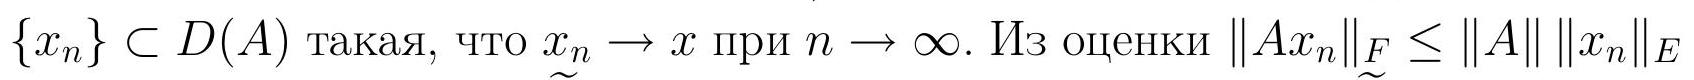
\includegraphics[width=\textwidth]{1}

при $n \rightarrow \infty$ получим $\|\widetilde{A} x\|_{F} \leq\|A\|\|x\|_{E}$. Таким образом, $\widetilde{A} \in L(E, F)$ и $\|\widetilde{A}\| \leq\|A\|$ Получим обратную оценку.
$$\|\widetilde{A}\|=\sup _{\substack{x \in E \\\|x\|_{E}=1}}\|\widetilde{A} x\|_{F} \geq \sup _{\substack{x \in D(A) \\\|x\|_{E}=1}}\|\widetilde{A} x\|_{F}=\sup _{\substack{x \in D(A) \\\|x\|_{E}=1}}\|A x\|_{F}=\|A\|.$$

Итак, $\|\widetilde{A}\|=\|A\| . \odot$

Построенный оператор $\widetilde{A}$ называют продолжением оператора $A$ nо непрерывности на все пространство.

\begin{itemize}
  \item ЗАДАЧА.
\end{itemize}

5.1. Пусть $H$ - гильбертово пространство и $M \subset H$ - линейное многообразие. Пусть $A$ - линейный ограниченный оператор, заданный на $M$ со значениями в банаховом пространстве $E$. Показать, что оператор $A$ можно продолжить на все пространство $H$ с сохранением нормы.

\section*{§6. Обратимый и обратный операторы}
Пусть $E, F$ - линейные нормированные пространства и $A$ - линейный (возможно неограниченный) оператор из $E$ в $F$, область определения $D(A) \subset E$ и множество значений $R(A) \subset F$, то есть $A: D(A) \subset E \rightarrow R(A) \subset F$.

Оператор $A$ называется обратимым, если

$$
(\forall y \in R(A))(\exists x \in D(A) \text { единственный })[A x=y] .
$$

Таким образом, в случае обратимого оператора $A$ определено отображение $A^{-1}$ из $F$ в $E$ с областью определения $D\left(A^{-1}\right)=R(A)$ и множеством значений $R\left(A^{-1}\right)=D(A)$ такое, что для $y \in R(A)$ определен $A^{-1} y=x$, где $x \in D(A)$ такой единственный, что $A x=y$.

Теорема 6.1. Пусть E,F - линейные нормированные пространства. Отображение $A^{-1}$, определенное по линейному обратимому оператору $A: D(A) \subset E \rightarrow R(A) \subset F$, является линейным оператором.

Доказательство. Напомним, что $D(A)$ и $R(A)$ являются линейными многообразиями в пространствах $E$ и $F$ соответственно.

Пусть выбраны элементы $y_{1}, y_{2} \in R(A)$ и числа $\alpha_{1}, \alpha_{2}$. Обозначим

$$
x_{1}=A^{-1} y_{1} \in D(A), \quad x_{2}=A^{-1} y_{2} \in D(A) \text {. }
$$

В силу линейности и обратимости оператора $A$ получим

$$
A\left(\alpha_{1} x_{1}+\alpha_{2} x_{2}\right)=\alpha_{1} y_{1}+\alpha_{2} y_{2} .
$$

Из определения отображения $A^{-1}$ следует

$$
A^{-1}\left(\alpha_{1} y_{1}+\alpha_{2} y_{2}\right)=\alpha_{1} x_{1}+\alpha_{2} x_{2}=\alpha_{1} A^{-1} y_{1}+\alpha_{2} A^{-1} y_{2} .
$$

Линейный оператор $A^{-1}$, определенный по линейному обратимому оператору $A$, называется оператором обратным к оператору $A$.

Из определения оператора $A^{-1}$ следует, что

$$
(\forall y \in R(A))\left[A A^{-1} y=y\right], \quad(\forall x \in D(A))\left[A^{-1} A x=x\right] .
$$

Для линейного оператора $A$ определим множество

$$
N(A)=\{x \in D(A) \mid A x=\Theta\}
$$

называемое ядром или нуль-многообразием оператора $A$. Нетрудно видеть, что $N(A)$ - линейное многообразие в пространстве $E$.

Теорема 6.2. Пусть E, F - линейные нормированные пространства и $A: D(A) \subset E \rightarrow F$ линейный оператор. Оператор $A$ обратим тогда $u$ только тогда, когда $N(A)=\{\Theta\}$.

Доказательство. Если оператор $A$ обратим, то уравнение $A x=\Theta \in R(A)$ имеет единственное решение $x=A^{-1} \Theta=\Theta \in D(A)$, то есть $N(A)=\{\Theta\}$.

Пусть теперь $N(A)=\{\Theta\}$. Предположим для $y \in R(A)$ существуют $x_{1}, x_{2} \in D(A)$ такие, что $A x_{1}=y$ и $A x_{2}=y$. Тогда $A\left(x_{1}-x_{2}\right)=\Theta$, что означает $x_{1}-x_{2} \in N(A)$. Следовательно, $x_{1}=x_{2}$. Итак, элемент $x \in D(A)$ такой, что $A x=y$ единственный. Значит оператор $A$ обратим. $\bigcirc$

Теорема 6.3. Пусть E, F - линейные нормированные пространства и $A: D(A) \subset E \rightarrow F$ линейный оператор. Оператор $A$ обратим и оператор $A^{-1}$ ограничен на $D(A)$ тогда и только тогда, когда

$$
(\exists m>0)(\forall x \in D(A))\left[\|A x\|_{F} \geq m\|x\|_{E}\right] .
$$

Доказательство. Пусть оператор $A$ обратим и оператор $A^{-1}$ ограничен на $D(A)$. Тогда

$$
(\exists C>0)(\forall y \in R(A))\left[\left\|A^{-1} y\right\|_{E} \leq C\|y\|_{F}\right]
$$

Возьмем произвольный $x \in D(A)$ и пусть $y=A x \in R(A)$. Тогда $x=A^{-1} y$ и $\|x\|_{E} \leq C\|A x\|_{F}$. Следовательно,

$$
(\exists C>0)(\forall x \in D(A))\left[\|A x\|_{F} \geq \frac{1}{C}\|x\|_{E}\right]
$$

Пусть теперь выполнено (6.1), из которого сразу следует $N(A)=\{\Theta\}$, то есть оператор $A$ обратим и существует обратный $A^{-1}$. Покажем ограниченность на $R(A)$ обратного оператора. Возьмем $y \in R(A)$ и $x=A^{-1} y \in D(A)$. Тогда из (6.1) $\|A x\|_{F} \geq m\|x\|_{E}$. Но $A x=y$, поэтому $\|y\|_{F} \geq m\left\|A^{-1} y\right\|_{E}$. Получили ограниченность на $R(A)$ оператора $A^{-1}$ и $\left\|A^{-1}\right\| \leq 1 / m$. $\odot$ Пусть $E, F$ - линейные нормированные пространства и линейный оператор $A: D(A) \subset E \rightarrow F$. 

Оператор $A$ называется непрерывно обратимым, если оператор $A$ обратим и обратный $A^{-1} \in L(F, E)$.

Лемма 6.1. Пусть $E, F$ - линейные нормированные пространства. Оператор $A \in L(E, F)$, и пусть существует оператор $B \in L(F, E)$ такой, что $B A=I_{E}$ и $A B=I_{F}$ (операторы $I_{E}$ и $I_{F}$ тождественные на E и $F$ соответственно). Тогда оператор $A$ непрерывно обратим и $A^{-1}=B$.

Доказательство. Пусть элемент $x \in N(A)$, то есть $A x=\Theta$. Следовательно, $x=I_{E} x=B A x=B \Theta=\Theta$. Получили $N(A)=\{\Theta\}$ и оператор $A$ обратим.

Возьмем $y \in F$. Тогда $y=I_{F} y=A B y=A(B y) \in R(A)$, то есть $R(A)=F$. Рассмотрим $A^{-1} y=A^{-1} A B y=B y$. Следовательно, $A^{-1}=B \in L(F, E)$. ○

Теорема 6.4. Пусть $E$ - банахово пространство и оператор $A \in L(E)$ такой, что $\|A\| \leq q<1$. Тогда оператор $I-A$ непрерывно обратим. Справедливо представление $(I-A)^{-1}=\sum_{k=0}^{\infty} A^{k}$ и оценка $\left\|(I-A)^{-1}\right\| \leq(1-q)^{-1}$.

Доказательство. Рассмотрим в $L(E)$ операторный ряд $\sum_{k=0}^{\infty} A^{k}$, где оператор $A^{0}=I$. Этот ряд сходится абсолютно, так как $\left\|A^{k}\right\| \leq\|A\|^{k} \leq q^{k}$, а числовой ряд $\sum_{k=0}^{\infty} q^{k}$ сходится. Так как $L(E)$ банахово пространство, то в $L(E)$ сходится и ряд $\sum_{k=0}^{\infty} A^{k}=S \in L(E)$.

Обозначим $\sum_{k=0}^{n} A^{k}=S_{n} \in L(E)$. Заметим, что $S_{n}(I-A)=I-A^{n+1}$. В последнем равенстве переходим к пределу при $n \rightarrow \infty$. Так как при $n \rightarrow \infty$

$$
\begin{gathered}
\left\|I-\left(I-A^{n+1}\right)\right\|=\left\|A^{n+1}\right\| \leq q^{n+1} \rightarrow 0, \\
\left\|S(I-A)-S_{n}(I-A)\right\| \leq\left\|S-S_{n}\right\|\|I-A\| \rightarrow 0,
\end{gathered}
$$

то в пределе получим $S(I-A)=I$. Аналогично доказывается $(I-A) S=I$.

Из леммы 6.1 теперь следует непрерывная обратимость оператора $I-A$ и $(I-A)^{-1}=S \in L(E)$. Получим необходимую оценку

$$
\left\|(I-A)^{-1}\right\|=\|S\|=\lim _{n \rightarrow \infty}\left\|S_{n}\right\| \leq \lim _{n \rightarrow \infty} \sum_{k=0}^{n}\left\|A^{k}\right\| \leq \sum_{k=0}^{\infty} q^{k}=(1-q)^{-1} .
$$

Замечание. Более сильное утверждение получается, если вместо условия $\|A\| \leq q<1$, обеспечивающего сходимость ряда $\sum_{k=0}^{\infty}\|A\|^{k}$, воспользоваться признаком Коши сходимости этого ряда $\lim _{k \rightarrow \infty}\left\|A^{k}\right\|^{1 / k}<1$. Известно (напр.,[8]), что такой предел $r(A)=\lim _{k \rightarrow \infty}\left\|A^{k}\right\|^{1 / k}$ существует и называется спектральным радиусом оператора $A$. Из определения спектрального радиуса $r(A)$ видно, что $r(A) \leq\|A\|$. Следствие 6.1. Пусть $E$ - банахово пространство, оператор $A \in L(E)$ и его спектральный радиус $r(A)<1$. Тогда оператор $I-A$ непрерывно обратим и справедливо представление $(I-A)^{-1}=\sum_{k=0}^{\infty} A^{k}$.

\begin{itemize}
  \item ЗАДАЧИ.
\end{itemize}

6.1. В пространстве $l_{2}$ рассмотрим операторы $A$ и $B$, переводящие элементы $x=\left(x_{1}, x_{2}, \ldots, x_{k}, \ldots\right)$ в $A x=\left(0, x_{1}, x_{2}, \ldots\right)$ и $B x=\left(x_{2}, x_{3}, \ldots\right)$ соответственно. Являются ли операторы $A$ и $B$ обратимыми ?

6.2. Рассмотрим оператор $A: C[0,1] \rightarrow C[0,1]$, заданный выражением

$$
A x(t)=\int_{0}^{t} x(s) d s
$$

а) Что представляет собой $R(A)$ ?

б) Существует ли обратный оператор и ограничен ли он ?

6.3. Показать, что соответствующие операторы $A: C[0,1] \rightarrow C[0,1]$ непрерывно обратимы и найти обратные:
a) $A x(t)=x(t)+\int_{0}^{t} x(s) d s$
б) $A x(t)=x(t)-\int_{0}^{1} t s x(s) d s$
в) $A x(t)=x(t)+\int_{0}^{1} \exp (t+s) x(s) d s$.

6.4. Пусть $E$ - линейное нормированное пространство и $A: E \rightarrow E$ такой линейный оператор, что ряд $\sum_{k=0}^{\infty} A^{k} x$ сходится для всех $x \in E$.

a) Доказать, что оператор $I-A$ обратим.

б) Пусть, кроме того, $A \in L(E)$. Доказать, что тогда для любого $x \in E$ выполнено $(I-A)^{-1} x=\sum_{k=0}^{\infty} A^{k} x$.

6.5. Пусть $E$ - банахово пространство, оператор $A \in L(E)$ и $\|I-A\|<1$. Доказать, что оператор $A$ непрерывно обратим.

6.6. Пусть $E$ - банахово пространство. Доказать, что в пространстве $L(E)$ множество всех непрерывно обратимых операторов открыто.

\section*{§ 7. Теорема Банаха об обратном операторе}
Теорема 7.1(Банах). Пусть $E, F$ - банаховы пространства. Пусть оператор $A \in L(E, F)$ такой, что $N(A)=\{\Theta\}$ u $R(A)=F$. Тогда оператор $A$ непрерывно обратим, то есть существует $A^{-1} \in L(F, E)$.

Обратим внимание, что существование оператора $A^{-1}: F \rightarrow E$ очевидно, так как $N(A)=\{\Theta\}$. Следует установить ограниченность оператора $A^{-1}$. Рассмотрим прежде вспомогательную лемму, при доказательстве которой существенно используются три простых факта, которые сформулируем в виде задач.

\begin{itemize}
  \item ЗАДАЧИ.
\end{itemize}

7.1. Пусть $E$ - линейное нормированное пространство и множество $M \subset E$. Тогда $(\forall \lambda-$ числа $)[\lambda \bar{M}=\overline{\lambda M}]$.

7.2. Пусть $E$ - линейное нормированное пространство и шар $B[x, r] \subset E$. Тогда $(\forall \lambda-$ числа $)[\lambda B[x, r]=B[\lambda x,|\lambda| r]]$.

7.3. Пусть $E$ - линейное нормированное пространство и шар $B[x, r] \subset E$. Тогда $B[x, r]-B[x, r]=B[\Theta, 2 r]$.

Лемма 7.1. Пусть $E$ - банахово пространство и $F$ - линейное нормированное пространство. Пусть задан линейный оператор $T: E \rightarrow F$ (возможно неограниченный). Определим множество $S=\left\{x \in E \mid\|T x\|_{F} \leq 1\right\}$. Тогда

$$
(\exists c>0)(\forall r>0)[B[\Theta, r] \subset \overline{r c S}]
$$

Доказательство. Для $k \in \mathbb{N}$ определим множества $k S=\{k x \mid x \in S\}$. Покажем, что $E=\cup_{k=1}^{\infty} k S$. Включение $\cup_{k=1}^{\infty} k S \subset E$ очевидно. Установим обратное включение. Пусть $x \in E$. Тогда $(\exists k \in \mathbb{N})\left[\|T x\|_{F} \leq k\right]$. Заметим, что $\|T(x / k)\|_{F} \leq 1$, то есть $x / k \in S$. Следовательно, $x=k(x / k) \in k S$. Установили $E \subset \cup_{k=1}^{\infty} k S$.

Так как пространство $E$ банахово, то $E$ есть множество второй категории, следовательно найдется множество $m S(m \in \mathbb{N})$, которое не является нигде не плотным. Таким образом,

$$
\left(\exists B\left(x_{0}, r_{0}\right) \subset E\right)\left(\forall B(x, \varepsilon) \subset B\left(x_{0}, r_{0}\right)\right)[B(x, \varepsilon) \cap m S \neq \varnothing]
$$

Итак, шар $B\left(x_{0}, r_{0}\right) \subset \overline{m S}$. Отсюда следует $B\left[x_{0}, r_{0}\right] \subset \overline{m S}=m \bar{S}$ (задача 7.1). Далее получим (задача 7.2)

$$
B\left[\frac{x_{0}}{m}, \frac{r_{0}}{m}\right]=\frac{1}{m} B\left[x_{0}, r_{0}\right] \subset \frac{1}{m}(m \bar{S})=\bar{S}
$$

Воспользуемся теперь задачей 7.3

$$
B\left[\Theta, 2 \frac{r_{0}}{m}\right]=B\left[\frac{x_{0}}{m}, \frac{r_{0}}{m}\right]-B\left[\frac{x_{0}}{m}, \frac{r_{0}}{m}\right] \subset \bar{S}-\bar{S} .
$$

Установим теперь, что $\bar{S}-\bar{S} \subset 2 \bar{S}$. Пусть элемент $z \in \bar{S}-\bar{S}$, то есть $z=x-y$, где $x, y \in \bar{S}$. Возьмем последовательности $\left\{x_{n}\right\},\left\{y_{n}\right\} \subset S$ такие, что $x_{n} \rightarrow x$ и $y_{n} \rightarrow y$ при $n \rightarrow \infty$. Тогда $z_{n}=x_{n}-y_{n} \rightarrow x-y=z$. Рассмотрим

$$
\left\|T z_{n}\right\|_{F}=\left\|T x_{n}-T y_{n}\right\|_{F} \leq\left\|T x_{n}\right\|_{F}+\left\|T y_{n}\right\|_{F} \leq 1+1=2 .
$$

В таком случае, $z_{n} \in 2 S$. Но тогда $z \in \overline{2 S}=2 \bar{S}$. Получили $B\left[\Theta, 2 r_{0} / m\right] \subset 2 \bar{S}$. Далее рассмотрим шар

$$
B[\Theta, 1]=\frac{m}{2 r_{0}} B\left[\Theta, \frac{2 r_{0}}{m}\right] \subset \frac{m}{2 r_{0}} 2 \bar{S}=\frac{m}{r_{0}} \bar{S} .
$$

Обозначим $m / r_{0}=c$. Итак, $B[\Theta, 1] \subset c \bar{S}$.

Теперь возьмем произвольное $r>0$ и получим

$$
B[\Theta, r]=r B[\Theta, 1] \subset r c \bar{S}=\overline{r c S}
$$

Доказательство теоремы 7.1. Как отмечалось выше, определен оператор $A^{-1}: F \rightarrow E$. Определим множество $P=\left\{y \in F \mid\left\|A^{-1} y\right\|_{E} \leq 1\right\}$. Возьмем произвольный шар $B[\Theta, r] \subset F$. Так как пространство $F$ банахово, то по лемме 7.1

$$
(\exists c>0)(\forall r>0)[B[\Theta, r] \subset \overline{r c P}]
$$

Пусть $y \in B[\Theta, 1] \subset F$. Так как $B[\Theta, 1] \subset \overline{c P}$, то найдется $y_{1} \in c P$, что $\left\|y-y_{1}\right\|_{F}<2^{-1}$. Так как $y-y_{1} \in B\left[\Theta, 2^{-1}\right] \subset \overline{2^{-1} c P}$, то найдется $y_{2} \in 2^{-1} c P$, что $\left\|\left(y-y_{1}\right)-y_{2}\right\|_{F}<2^{-2}$. Элемент $y-y_{1}-y_{2} \in B\left[\Theta, 2^{-2}\right] \subset \overline{2^{-2} c P}$, поэтому найдется $y_{3} \in 2^{-2} c P$, что $\left\|\left(y-y_{1}-y_{2}\right)-y_{3}\right\|_{F}<2^{-3}$ и так далее.

По построению для всех $i \in \mathbb{N}$ элементы $y_{i} \in 2^{1-i} c P$, следовательно, $\left\|A^{-1} y_{i}\right\|_{E} \leq c 2^{1-i}$. Кроме того, $\left\|y-\sum_{i=1}^{k} y_{i}\right\|_{F}<2^{-k} \rightarrow 0$ при $k \rightarrow \infty$. Следовательно, $y=\sum_{i=1}^{\infty} y_{i}$.

Обозначим $x_{i}=A^{-1} y_{i}$. Рассмотрим в $E$ ряд $\sum_{i=1}^{\infty} x_{i}$. Этот ряд абсолютно сходится, так как $\sum_{i=1}^{\infty}\left\|x_{i}\right\|_{E} \leq c \sum_{i=1}^{\infty} 2^{1-i}=2 c$. Пространство $E$ банахово, поэтому $\sum_{i=1}^{\infty} x_{i}=x \in E$. В силу непрерывности оператора $A$ получим

$$
A x=\sum_{i=1}^{\infty} A x_{i}=\sum_{i=1}^{\infty} y_{i}=y
$$

В таком случае, $x=A^{-1} y$ и

$$
\left\|A^{-1} y\right\|_{E}=\|x\|_{E}=\left\|\sum_{i=1}^{\infty} x_{i}\right\|_{E} \leq \sum_{i=1}^{\infty}\left\|x_{i}\right\|_{E} \leq 2 c .
$$

Из последней оценки следует $\left\|A^{-1}\right\| \leq 2 c$, то есть $A^{-1} \in L(F, E) . \odot$

\begin{itemize}
  \item ЗАДАЧА.
\end{itemize}

7.4. Пусть на линейном пространстве $E$ заданы две нормы: $\|x\|_{1}$ и $\|x\|_{2}$. По отношению к каждой из них $E$ полное пространство. Предположим, что $(\exists c>0)(\forall x \in E)\left(\|x\|_{1} \leq c\|x\|_{2}\right)$. Доказать, что нормы $\|x\|_{1}$ и $\|x\|_{2}$ эквивалентны.
\end{document}